\documentclass[11pt]{report}
\usepackage[margin = 1in]{geometry}              
\geometry{a4paper}                  
\usepackage[parfill]{parskip}    
\usepackage{fancyhdr}
\usepackage{enumitem}
\usepackage{longtable}
\usepackage{amsmath}
\usepackage{minted}
\usepackage{listings}
\usepackage{framed}
\usepackage{graphicx}
\usepackage[toc,page]{appendix}
\usepackage{lscape}
\usepackage{rotating}

\title{Assignment \#1 - Lotka-Volterra Dynamical Systems}   
\date{\today}
\pagestyle{fancyplain}
\author{Jonathan Rainer}

\begin{document}
	\fancyhf{}
	\lhead{Jonathan Rainer}
	\chead{\thepage}
	\rhead{\today}
	\renewcommand{\headrulewidth}{0.3pt}
	\renewcommand{\footrulewidth}{0.3pt}
	\maketitle
	
	\chapter*{Question \#1}
	Consider the simple nonlinear dynamical system (the "Lotke-Volterra predator-prey system")
	$$
	x' = \dfrac{dx}{dt} = ax - bxy ; \quad y' = \dfrac{dy}{dt} = cxy - dy
	$$
	where $x$ and $y$ are the population densities of predators and prey respectively. In addition $a$, $b$, $c$, $d$ are strictly positive constants.
	\begin{enumerate}[label=\alph*)]
		\item 
			\begin{enumerate}[label=\roman*)]
				\item Define a MATLAB function \texttt{lvderivs} to evaluate the time derivatives for this dynamical system, taking care to define any parameters as \texttt{global} if necessary.
				
				The function that answers this question can be seen in Figure \ref{fig:lvderivs}.
				
				\item Verify that the origin (0,0) is a trivial fixed point of the dynamical system by evaluating \texttt{lvderivs} at this point.
				
				To verify this we simply need to execute the function defined for the derivatives and show that the output is indeed $[0,0]$, as Figure \ref{fig:lvderivs_trivial_output}.
				
				\begin{figure}[h]
					\begin{framed}
						\begin{verbatim}
						>> lvderivs([0,0])
						
						ans =
						
							 0     0
						\end{verbatim}
					\end{framed}
					\caption{The evaluation of the lvderivs function at the point $[0,0]$ as copied from the MATLAB command window}
					\label{fig:lvderivs_trivial_output}
				\end{figure}
				
			\end{enumerate} 
		\item
			\begin{enumerate} [label=\roman*)]
				\item Write a MATLAB script which uses \texttt{fsolve} with your \texttt{lvderivs} function and range of random (physically reasonable) initial guesses to show that the system has a strictly positive fixed point. 
				
				The first thing that would make sense in this case would be to look at the dynamics phase portrait to see what the physically reasonable guesses might be in this case. This can be seen in Figure \ref{fig:phase_plane} with the code that produced the diagram shown in Figure \ref{fig:phase_plane_plotting_code}. 
				
				\begin{figure}[h]
					\begin{center}
						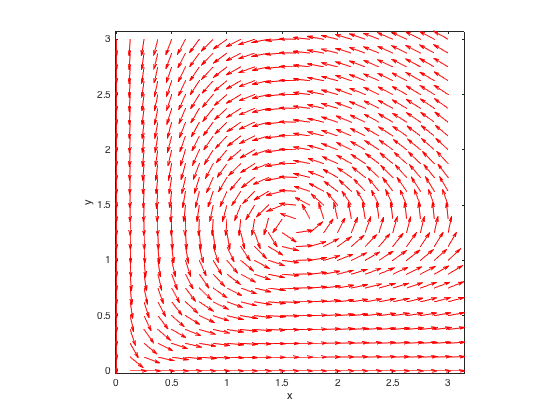
\includegraphics[width=5in, clip]{phase_plane.png}
					\end{center}
					\caption{The phase plane for the given equations, plotted between $0$ and $3$. This shows that anything between 0 and 2 will probably converge to a root as we require}
					\label{fig:phase_plane}
				\end{figure}
				
				From this it would appear that we have at least one other fixed point than the trivial point already found and we know this to be true because of the following reasoning. If we look at the nullclines for $\dfrac{dx}{dt}$ we see the following:
				
				$$
				0 = \dfrac{dx}{dt} = ax-bxy \implies 0 = x(a-by) \implies x = 0 \text{ or } y = \dfrac{a}{b}
				$$
				
				And then if we look at the nullclines for $\dfrac{dy}{dt}$ then we can also see the following:
				
				$$
				0 = \dfrac{dy}{dt} = cxy - dy \implies 0 = y(cx - d) \implies y = 0 \text{ or } x = \dfrac{d}{c}
				$$
				
				Now the fixed points will be the intersections of these solutions, so we'll get one from $x=0 $, $y=0$ crossing over and then one from the non-trivial solutions crossing since all these are linear equations. So we know we're looking for two fixed points.
				
				Now we can turn our attention to finding the fixed points, which is done by repeatedly iterating \texttt{[text]}fsolve for a variety of random starting values between $(0,0)$ and $(2,2)$ as we know the fixed points lie in those regions from observing the phase portrait. This obviously not infallible and relies on knowing how many fixed points there are in advance but it does provide a reasonable way of attempting to find as many as possible, and allows similarity thresholds which can be tuned so the output resembles what we see in the qualitative phase portrait. The output produced by the function can be seen below in Figure \ref{fig:equilibria_finder_output} with the code that produced the output shown in Figure \ref{fig:equilibria_finder_code}.
				
				\begin{figure}[h]
					\begin{framed}
						\begin{verbatim}
						>> eqi = equilibria_finder(100, 0.00001, 0.00001, 5, 0, 2)
						
						eqi = 
						
						[1x2 double]
						[1x2 double]
						
						>> celldisp(eqi)
						
						eqi{1} =
						
						0     0
						
						eqi{2} =
						
						1.6000    1.3333
						
						>> lvderivs(eqi{1})
						
						ans =
						
						1.0e-06 *
						
						-0.3497    0.2331
						\end{verbatim}
					\end{framed}
					\caption{The output from the MATLAB command window when running the defined functions, plus some code to display the fixed points. In addition we numerically verify that the points found are indeed fixed points by running them back through the derivative function.}
					\label{fig:equilibria_finder_output}
				\end{figure}
				
				\item Find the eigenvalues of the system's Jacobian matrix at this strictly positive fixed point.
				
				This question is relatively easy because we can use the solutions we've already found from the previous part and then use another output from \texttt{fsolve} to find Jacobian as shown in Figure \ref{fig:jacobian_output}.
				
				\begin{figure}[h]
					\begin{framed}
						\begin{verbatim}
						>> eqi = equilibria_finder(100, 0.00001, 0.00001, 5, 0, 2)
						
						eqi = 
						
						[1x2 double]
						[1x2 double]
						
						>> eqi{1}
						
						ans =
						
						1.6000    1.3333
						
						>> [~,~,~,~,J] = fsolve(@lvderivs,eqi{1})
						
						J =
						
						-0.0000   -1.2000
						0.6667    0.0000
						
						>> eig(J)
						
						ans =
						
						-0.0000 + 0.8944i
						-0.0000 - 0.8944i
						
						\end{verbatim}
					\end{framed}
					\caption{The output from the MATLAB command window when using \texttt{fsolve} to extract the Jacobian and find its eigenvalues.}
					\label{fig:jacobian_output}
				\end{figure}
				So now we know that the Jacobian is as follows:
				$$
				J = \begin{bmatrix} 
					0 & -1.2 \\
					0.6667 & 0
					\end{bmatrix}
				$$
				Consequently $J$ is diagonal so we can simply read the eigenvalues from the matrix. Thus the eigenvalues are $\lambda_1 = 0.8944i$ and $\lambda_2 = -0.8944i$
				
			\end{enumerate}
		\item Using \texttt{ode45} to integrate the system forward in time, using a range of initial values with $x$-co-ordinate on the non-trivial $y$ null-cline $x = \frac{d}{c}$ and using a time interval appropriate to reveal the system's dynamics.
		
		The best way to solve this question is to use \texttt{ode45} with some of the phase plane tools we've already built up in trying to solve the previous questions. Using this we can generate several plots over increasing time spans and use that to develop an understanding of the system as a whole. So in the first instance we can use the script seen in Figure \ref{fig:plotting_code} to generate the nine plots seen in Figure \ref{fig:ode45_plots}. These seem to be showing some kind of oscillatory behaviour, now if we plot the same behaviour within the phase portrait this will give us another idea of the dynamics and this can be seen in Figure \ref{fig:phase_plots}. The code used to produce each individual plot can seen in Figure \ref{fig:phase_portrait_trajectories_code}, and the a script to automate seen in Figure \ref{fig:multi_phase_portrait_plotting_code}. All this together indicates that the dynamics around around the non-trivial fixed point are essentially oscillatory (i.e the fixed point is unstable) but decaying very slowly out from the fixed point itself.
		
		\begin{sidewaysfigure}[ht]
				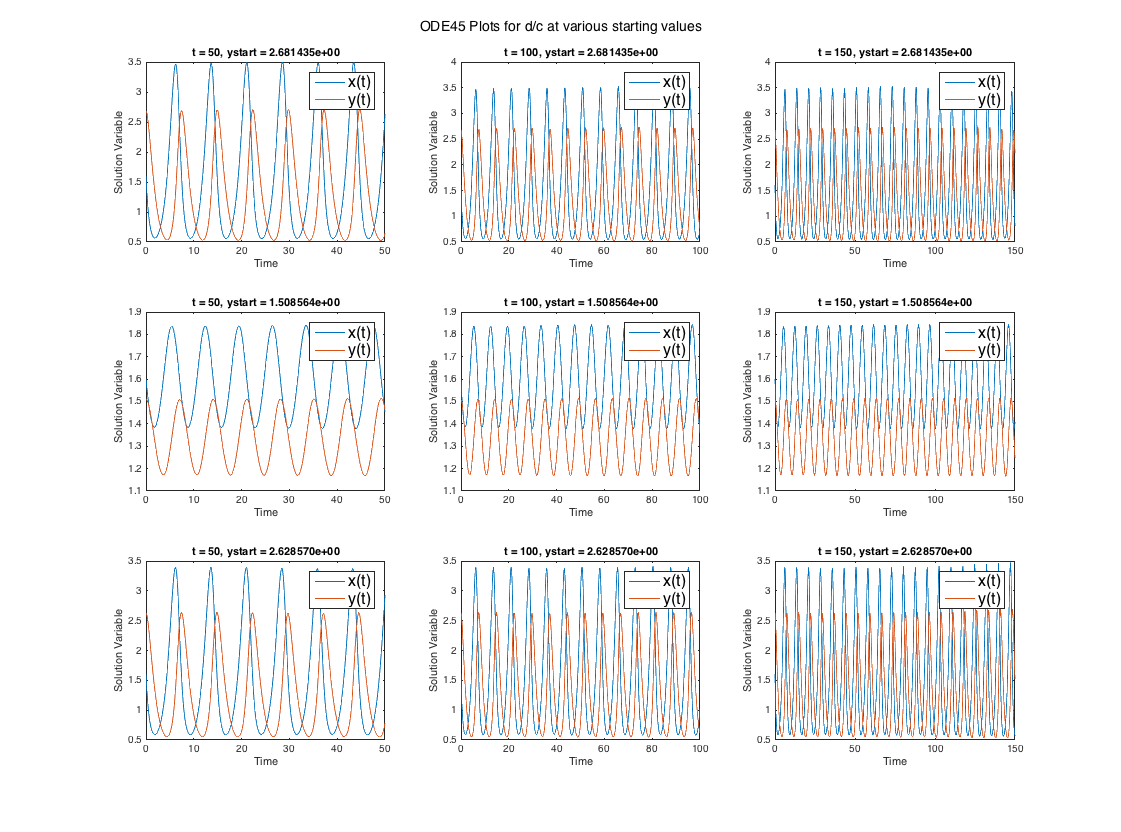
\includegraphics[width=9.8in]{ode45_plots.png}
				\caption{A selection of 9 plots done for different starting values of $y$ over increasing time spans. The behaviour shown seems to be in some sense oscillatory as we'll see later in the phase portraits}
				\label{fig:ode45_plots}
		\end{sidewaysfigure}
		
		\begin{sidewaysfigure}[ht]
			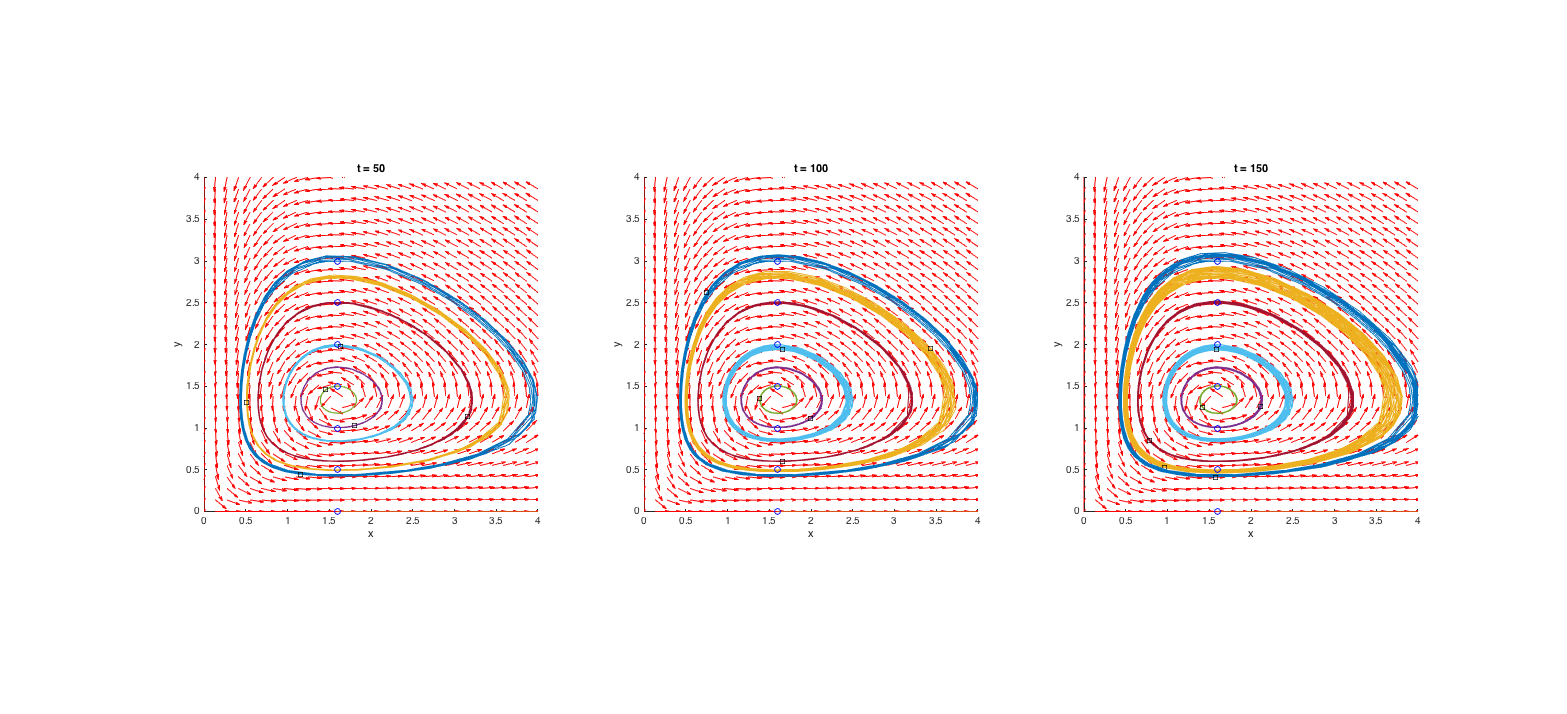
\includegraphics[width=10in]{phase_plots_trajectories.png}
			\caption{A selection of 3 plots done over the same starting y-values but with increasing time spent, the result is very similar to what we observe plotting the time series against time. An oscillatory behaviour around the non-trivial fixed point.}
			\label{fig:phase_plots}
		\end{sidewaysfigure}
		
		\item 
			\begin{enumerate}[label=\roman*)]
				\item Write your own MATLAB script (not a pre-defined function) which uses \texttt{lvderivs} to produce approximate solutions to the dynamical system using an explicit Euler method with a fixed time step, showing outputs for at least two different (fixed) time steps.
				
				The MATLAB code that solves this problem can be seen in Figure \ref{fig:euler_method_code} and the plots produced can be seen below in Figure \ref{fig:ode45_euler_compare_plot}. The code that produced these plots can be seen in Figure \ref{fig:euler_ode45_compare_code}.
				
				\begin{sidewaysfigure}[ht]
					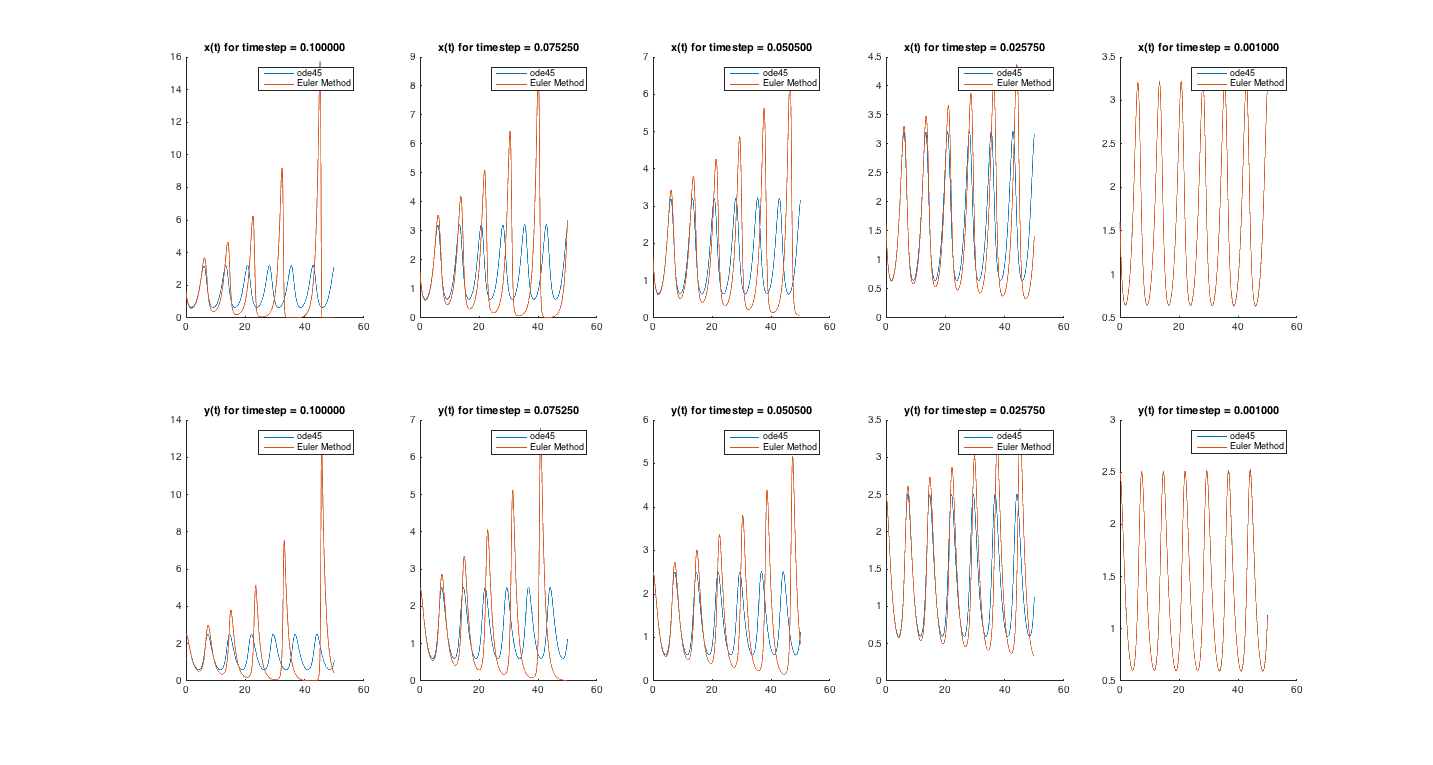
\includegraphics[width=10in]{ode45_euler_compare_plots.png}
					\caption{A selection of plots showing the effect of decreasing the step size in the Euler method using \texttt{ode45} as a comparison.}
					\label{fig:ode45_euler_compare_plot}
				\end{sidewaysfigure}
				
				\item Explain why these solutions differ to those of part c)
				
				As can be seen from the Figure [??] the reason for the difference lies in the choice of time step used to estimate the solution to the equations. As the time step gets shorter the estimated solutions gets much closer to \texttt{ode45}'s solution and the reason for this is because Euler's method relies on the idea that the function itself doesn't change a great deal within the interval described by each time step. If the function is quite erratic as the solutions to the dynamical system are the changes predicted will no line up with what actually happens in the system. Add to that the fact that the method is iterative so any error added will accumulated across multiple calculations and you end up with a situation like we see in the first set of figures. It's important to choose a step size that takes into account the erratic nature of the graph and from there can give an accurate representation of the behaviour of the function to be estimated.
				
			\end{enumerate}
	\end{enumerate}
	
	
	
	\chapter*{Question \#2}
	The Lotka-Volterra model in question 1 has been criticised because it does not have a linearly stable strictly positive equilibrium.
		\begin{enumerate}[label=\alph*)]
			\item 
				\begin{enumerate}[label=\roman*)]
					\item Modify the model so that, at least for some set of biological meaningful parameter values, it has a linearly stable strictly positive equilibrium. 
					
					The model will be modified to limit the growth of the prey population (more is explained in the next part). Suffice to say that the modification is to replace the exponential growth term in the current model with the logistic equation thus:
					
					$$
					x' = \dfrac{dx}{dt} = ax\left(1-\dfrac{x}{K}\right) - bxy ; \quad y' = \dfrac{dy}{dt} = cxy - dy
					$$
					
					Where $K$ is the carrying capacity of the population of prey.
					
					\item Explain what the modification represents biologically.
					
					Biologically this means that you're getting rid of the odd assumption that in the absence of a predator species the prey will grow without limit. With this modification it takes into account the fact that the environment within which the prey live can only support up to a certain amount of prey and so saturates the first term at this carrying capacity $K$. In other words if the population grows beyond the limit set by $K$ then the rate of change evaluates to a negative amount so the population cannot grow beyond the size of $K$. This introduces a linearly stable fixed point which points to the co-existence of both species under this model.
					
				\end{enumerate}
			\item Show either algebraically or numerically that there is a linearly stable strictly positive equilibrium in your revised model.
			
			Using the machinery we've already established we can fairly easily show that the equilibrium required does indeed exist. In the first instance if we form the equations for the $\dot{x}$ null-clines we see the following:
			
			$$
			0 = ax\left(1-\dfrac{x}{K}\right) - bxy \implies x\left(a-\dfrac{ax}{K} - by\right) = 0 \implies x = 0 \quad \text{ or} 
			$$
			$$
			\left(a-\dfrac{ax}{K} - by\right) = 0 \implies bKy = aK-ax \implies y = \frac{a}{b} - \frac{ax}{bK} = \dfrac{a}{b}\left(1-\frac{x}{K}\right)
			$$
			
			and similarly for the $\dot{y}$ null-clines:
			
			$$
			0 = cxy - dy = y(cx -d) \implies y = 0 \quad \text{ or } \quad x = \frac{d}{c}
			$$
			
			Now the fixed points are at $(0,0)$ and $\left(\dfrac{d}{c}, \dfrac{a}{b}\left(1-\dfrac{d}{Kc}\right)\right)$
			
			Now the Jacobian is the following 
			
			$$
			J(x,y) = \begin{bmatrix}
				a(1-x) - \dfrac{2ax}{K}-by & -bx \\
				cy & cx - d 
			\end{bmatrix}
			$$
			
			Now the first thing to spot is if we evaluate this at the non-trivial fixed point the bottom right entry will be 0. Which means that the trace will only recieve a contribution from the upper left term. Now if we evaluate this we see the following:
			
			$$
			a\left(1 - \frac{d}{c}\right) - \dfrac{2ad}{cK} - a\left(1-\dfrac{d}{Kc}\right) = a - \dfrac{ad}{c} - \dfrac{2ad}{cK} - a + \dfrac{ad}{cK} = -\dfrac{ad}{c}\left(1 + \dfrac{1}{K}\right)
			$$
			
			Now this term will always be negative due to the restrictions on the constants we can choose. So we'll always have a strictly negative trace. Now considering the determinant we know that because the bottom right entry is $0$ the determinant $\Delta$ is equal to $bcxy$. Now since $x$ and $y$ are both positive as this system models physical phenomena this term is positive so we have a positive determinant and a negative trace which leads to the fixed point is stable for any choice of parameter values. This can be seen from the plot included below in Figure \ref{fig:linearly_stable_plot} which shows several trajectories converging onto the non-trivial stable fixed point, plotted using the same tools as the other phase plots but with a new derivative function.
			
			\begin{figure}[h]
				\begin{center}
					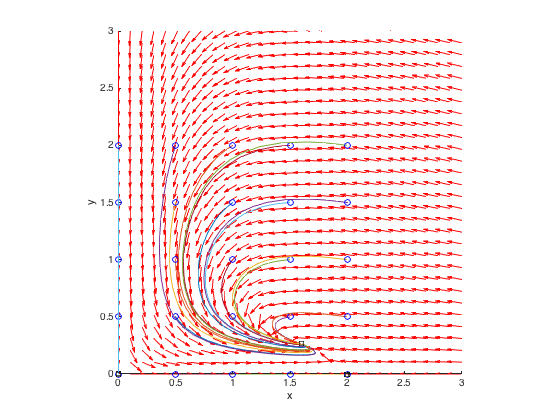
\includegraphics[width=5in]{linearly_stable_fixed_point_plot.png}
				\end{center}
				\caption{A plot for the new dynamical system with chosen parameter values, showing that all the trajectories converge to the stable fixed point, indicating a co-existence of the two species.}
				\label{fig:linearly_stable_plot}
			\end{figure}
			
			\item 
				\begin{enumerate}[label=\roman*)]
					\item Using a numerical method, calculate the elasticity of the linearly stable strictly positive equilibrium point, for some chosen set of parameter values.
					
					
					
					\item If possible, confirm your result numerically.
				\end{enumerate} 
			
		\end{enumerate}
	\begin{appendices}
		\chapter{Programming Code}
		
		\begin{figure}[h]
			\begin{framed}
				\inputminted[]{matlab}{../lvderivs.m}
			\end{framed}
			\caption{The definition of the \texttt{lvderivs} function is relatively simple it just sets up the parameters, factors out some recurring parts and then computes the derivatives.}
			\label{fig:lvderivs}
		\end{figure}
		
		\begin{figure}[h]
			\begin{framed}
				\begin{center}
					\inputminted[]{matlab}{../phase_portrait.m}
				\end{center}
			\end{framed}
			\caption{The code to generate the phase portrait displayed in Figure \ref{fig:phase_plane}. The code simply generates the required vectors and then computes the rate of change at each point and uses the quiver command to automate all the plotting.}
			\label{fig:phase_plane_plotting_code}
		\end{figure}
		
		\begin{figure}[h]
			\begin{framed}
				\begin{center}
					\inputminted[]{matlab}{../equilibria_finder.m}
				\end{center}
			\end{framed}
			\caption{This code simplifies repeatedly running \texttt{fsolve} but also allows us to check for duplicates when the repeated runs are aggregated. The secondary function allows for this by checking whether what exists is within a similarity threshold and if so ignoring it as a new fixed point. This allows us to account for the situation where you get several roots occuring within a very small interval. This option can be removed by setting the threshold to 0 of course.}
			\label{fig:equilibria_finder_code}
		\end{figure}
		
		\begin{figure}[h]
			\begin{framed}
				\begin{center}
					\inputminted[]{matlab}{../generate_ode45_plots.m}
				\end{center}
			\end{framed}
			\caption{This code automates the plotting of several ODE45 outputs, over multiple time spans and multiple initial starting values of $y$, the $x$-coordinate already being fixed to lie on the given null-cline.}
			\label{fig:plotting_code}
		\end{figure}
		
		\begin{figure}[h]
			\begin{framed}
				\begin{center}
					\inputminted[]{matlab}{../phase_portrait_trajectories.m}
				\end{center}
			\end{framed}
			\caption{This code automates the plotting of a phase portrait with the associated trajectories, it also uses ODE45 and marks the beginning and end of the trajectories as it appears on the diagram.}
			\label{fig:phase_portrait_trajectories_code}
		\end{figure}
		
		\begin{figure}[h]
			\begin{framed}
				\begin{center}
					\inputminted[]{matlab}{../generate_phase_plots.m}
				\end{center}
			\end{framed}
			\caption{This code simply automates the plotting of multiple phase portraits using the \texttt{subplot} commands.}
			\label{fig:multi_phase_portrait_plotting_code}
		\end{figure}
		
		\begin{figure}[h]
			\begin{framed}
				\begin{center}
					\inputminted[]{matlab}{../euler_method.m}
				\end{center}
			\end{framed}
			\caption{This code is an implementation of the Euler method which first sets the starting values in a matrix and then iterates finding the derivative and predicting the next point in the function.}
			\label{fig:euler_method_code}
		\end{figure}
		
		\begin{figure}[h]
			\begin{framed}
				\begin{center}
					\inputminted[]{matlab}{../compare_euler_ode45.m}
				\end{center}
			\end{framed}
			\caption{This code automates plotting the Euler approximation against the \texttt{ode45} output to see how they compare for decreasing step size.}
			\label{fig:euler_ode45_compare_code}
		\end{figure}
		
		\begin{figure}[h]
			\begin{framed}
				\begin{center}
					\inputminted[]{matlab}{../new_lvderivs.m}
				\end{center}
			\end{framed}
			\caption{This code calculates the new derivative function with the added carrying capacity scaling to introduce the linearly stable fixed point.}
			\label{fig:new_lvderivs_code}
		\end{figure}
		
		
	\end{appendices}
\end{document}
